\documentclass[10pt, journal]{IEEEtran}

\usepackage{url}
\usepackage{cite}
\usepackage{amsmath,amssymb,amsfonts}
\usepackage{algorithmic}
\usepackage{graphicx}
\usepackage{textcomp}
\usepackage{xcolor}
\usepackage{tikz}
\usepackage[section]{placeins}
\usepackage[justification=centering]{caption}
\usepackage{calc}
\usepackage[nomessages]{fp}
    
\usepackage[T1]{fontenc} % optional
\usepackage[cmintegrals]{newtxmath}
\usepackage{bm} % optional

\usepackage{glossaries}

\usetikzlibrary{shapes, arrows}

\makeatletter
\def\@hex@@Hex#1%
 {\if a#1A\else \if b#1B\else \if c#1C\else \if d#1D\else
  \if e#1E\else \if f#1F\else #1\fi\fi\fi\fi\fi\fi \@hex@Hex}
\makeatother

%\makeatletter
%\AtBeginDocument{%
%  \expandafter\renewcommand\expandafter\subsection\expandafter{%
%    \expandafter\@fb@secFB\subsection
%  }%
%}
%\makeatother

\makeglossaries
\loadglsentries{glsEntries}

%\usetikzlibrary{external}
%\tikzexternalize % activate!

\newlength{\smallColumnWidth}
\setlength{\smallColumnWidth}{\columnwidth-2cm}%


\definecolor{cCyan}{HTML}{8dd3c7}
\definecolor{cYellow}{HTML}{ffffb3}
\definecolor{cFlieder}{HTML}{bebada}
\definecolor{cRed}{HTML}{fb8072}
\definecolor{cBlue}{HTML}{80b1d3}
\definecolor{cOrange}{HTML}{fdb462}
\definecolor{cGreen}{HTML}{b3de69}
\definecolor{cPink}{HTML}{fccde5}

\title{Dynamic Partial Self-Reconfiguration of \\Self-Aware Systems for Fault Tolerance}
%\author{Constantin Schieber, 01228774}

\author{\IEEEauthorblockN{Constantin Schieber}
\IEEEauthorblockA{%\\Vienna University of Technology\\
\\Institute of Computer Technology\\
TU Wien, Vienna, Austria\\
Constantin.Schieber@tuwien.ac.at}
\thanks{This paper was prepared under the supervision of Dr. Nima TaheriNejad.}
}
\begin{document}
\maketitle

\begin{abstract}
    A system can be described as fault-tolerant if it can continue at the same level of performance even though one or more components have failed. 
    This property is inherently important for systems that operate without any chance of maintenance.
    \glspl{FPGA} provide the opportunity of \gls{DPR}, which provides them with the ability to efficiently react to faults that are introduced through environmental (e.g. radiation, heat) or internal (e.g. a malicious \gls{IP}) changes.
    Through the structural adaptions that are possible with \gls{DPR}, faulty chip areas can be avoided and a graceful degradation of performance with high granularity in reply to power constraints is possible.
    It also enables efficiency through selective instantiation of needed functionality.
    
    This work focuses on fault mitigation aspects of such systems. 
    It includes reviews of the types of faults that occur, methods for their detection and how certain faults can be mitigated. 
    We show that there is a wide variety of research on this topic that is especially mature in the aeronautics and space sector.
    Particularly the mitigation of faults within \glspl{FPGA} is widely researched.
    We also find that \gls{DPR} is rarely used to replace the functionality of external modules although this approach seems to provide a good base for economical redundancy solutions.
    \gls{DPR}, in general, enables a fault mitigation solution on the architectural level that enables the usage of commercial off-the-shelf hardware for uses under extreme conditions.
    
    % === Improved Version === %
    %We describe a system as fault-tolerant if it can continue at the same level of performance even though one or more components have failed.
    %This property is inherently important for systems that operate without any chance of maintenance.
    %Environmental (e.g. radiation, heat) or internal (e.g. a malicious \gls{IP}) changes are common causes for faults in hardware.
    %On \glspl{FPGA} we have the opportunity to use \gls{DPR}, which provides us with the ability to efficiently react to these faults.
    %The system can avoid faulty chip areas on the \gls{FPGA} with the help of \gls{DPR} by making structural adaptions.
    %This allows the system to gracefully degrade performance with a high granularity. 
    %It can consider and respect constraints like computing speed, power consumption and area usage during the degradation process.
    %It also increases efficiency through selective instantiation of needed functionality.
    
    %This work focuses on fault mitigation aspects of such systems. 
    %It includes reviews of the types of faults that occur, methods for their detection and how a system can mitigate certain faults. 
    %We show that there is a wide variety of research on this topic that is especially mature in the aeronautics and space sector.
    %Particularly the mitigation of faults within \glspl{FPGA} is widely researched.
    
    %We also find that \gls{DPR} is rarely used to replace the functionality of external modules although this approach seems to provide a good base for economical redundancy solutions.
    %\gls{DPR}, in general, enables a fault mitigation solution on the architectural level that enables the usage of commercial off-the-shelf hardware for uses under extreme conditions.
\end{abstract}

%\tableofcontents

\section{Introduction}\label{Introduction}
\glspl{FPGA} provide us with flexible options to reconfigure functionality at run-time. 
This flexibility can be exploited to increase fault resistance which in turn reduces the need for hardware redundancy. 

\gls{DPR} for fault mitigation can be split into two major fields of appliances. 
The first field discusses the mitigation of faults that occur within the \gls{FPGA}.
These faults interfere with the intended functionality of the tasks executed on the \gls{FPGA} itself, e.g. permanent and transient faults. 
The second area focuses on the mitigation of faults that are present in external devices by the provision of redundancy in the form of the \gls{FPGA}.
In the following, this work will refer to these two types of faults as \textit{internal} and \textit{external} faults, respectively.

The rest of this work is organized as follows.
A general overview over the existing literature and its main methodologies is given in \ref{sec:literatureOverview}.
Section \ref{InternalFaults} introduces different types of internal faults and a generally applicable fault mitigation flow in the context of \gls{DPR}.
After this, different architectures and strategies for fault mitigation with \gls{DPR} are introduced in Section \ref{InternalFaultsArch}.
This involves architectures that focus solely on the aspect of moving functionality from faulty to healthy tiles as well as solutions like \glspl{NoC}, that come with built in fault tolerance. 
For \glspl{NoC}, first we cover a security relevant scenario where faults are introduced with malicious intent by a third party through partial reconfiguration of a modified \glspl{IP}.
Second, we show how \glspl{NoC} can deal with internal faults that affect routing within the network.  
Section \ref{ExternalFaults} describes scenarios where external faults may happen and how they can be mitigated with the usage of minimal hardware resources. 
Section \ref{Conclusion} gives concluding remarks on the surveyed applications and an estimate on future developments.


\section{Literature Overview}\label{sec:literatureOverview}
Table \ref{tbl:literatureOverview} gives an overview over the existing literature and tries to classify the existing work by the used \textit{Fault Mitigation Method} and the \textit{Fault Detection Method}.
One can see that the prevalent strategy for Fault Mitigation is the \textit{Spare Tile Architecture}. 
This makes sense, as it is straight forward to implement with most of the standard vendor tool-chains.
An architecture was classified as \textit{Spare Tile Architecture} if it was reserving extra space for potentially occurring faults, consequently moving a faulty module to the healthy extra space.
Designs with this architecture mostly utilize \gls{TMR} as a \textit{Fault Detection Method} as it is easy and reliable to move a faulty module to the reserved space without compromising functionality.
Furthermore, these solutions can handle transient and permanent faults equally well.
The disadvantage of these methods in general is that they introduce an overhead in terms of used resources and storage for partial bitstreams.
Solutions to this are introduced in Section \ref{sec:SpareTileArchitecture}. 
They are also inflexible or at least not easy to generalize.

A solution to this is introduced with the \textit{Task Based Architecture}.
These architectures focus on a \gls{RTOS} based approach, where resilient modules are modelled as tasks that may be placed anywhere, anytime within the \gls{RP}. 
The listed works don't focus on fault detection, as it should be managed on the level of the \gls{RTOS}.
With a standardized communication interface and an OS-like scheduler, faults can be mitigated by re-scheduling modules to healthy tiles as needed. 
This makes the approach much more general, albeit it may compromise hard real-time requirements.

\glspl{NoC} already heave the inherent property of a standardized communication interface which may also be utilized to increase fault tolerance.
Re-routing of data-paths to avoid faulty or malicious nodes proves to be a useful means for handling transient and permanent faults.

Localized scrubbing is used to reduce scrubbing times, but requires the development of non-vendor tools and the modification of partial reconfiguration controllers.
It profits from a finer grained localization of faults.
While this approach reduces resource usage, it is not able to handle permanent faults. 

\begin{table*}
    \caption{Literature on the usage of \gls{DPR} for fault-tolerance.}
    \label{tbl:literatureOverview}
    \begin{tabular*}{\textwidth}{@{\extracolsep{\fill}}lll}
        \toprule
       \textbf{Authors} & \textbf{Fault Mitigation Method} & \textbf{Fault Detection Method} \\
       \midrule
       \cite{bolchini2007} Bolchini et al. 2007             & Spare Tile Architecture      & TMR  \\
       \cite{kastil2012} Kastil et al. 2012                 & Spare Tile Architecture      & TMR, DWC, CED  \\
       \cite{zhang2013} Zhang et al. 2013                   & Spare Tile Architecture      & Not specified \\
       \cite{dicarlo2014} Dicarlo et al. 2014               & Spare Tile Architecture      & Error Signals, Tests \\
       \cite{davis2014} Davis et al. 2014                   & Spare Tile Architecture      & Algorithm Based Fault Tolerance \\
       \cite{lameres_radsat_2015} LaMeres et al. 2015       & Spare Tile Architecture      & TMR  \\
       \cite{martins_tmr_2015} Martins et al. 2015          & Spare Tile Architecture      & TMR  \\
       \cite{wilson_hybrid_2017} Wilson et al. 2017         & Spare Tile Architecture      & TMR  \\
       \cite{martins_dynamic_2018} Martins et al. 2018      & Spare Tile Architecture      & TMR  \\
       \cite{wang_dynamic_2018} Wang et al. 2018            & Task Based Architecture      & Scrubbing \\
       \cite{sharma_run-time_2018} Sharma et al. 2018       & Task Based Architecture      & - \\
       \cite{kadri_survey_2019} Kadri et al. 2019           & NoC - Routing, Remapping, Redundancy                        & - \\
       \cite{wehbe_secure_2016} Wehbe et al. 2016           & NoC - Routing               & Timeout\\
       \cite{frenkel2015} Frenkel et al. 2015               & Localized Scrubbing       & Forward Temporal Redundancy \\
       \cite{nunes_improving_2016} Nunes et al. 2016        & Localized Scrubbing         & - \\
       \cite{kourfali2019} Kourfali et al. 2019             & Localized Scrubbing           & TMR \\
       \cite{zhao_fine-grained_2018} Zhao et al. 2018       & Fine grained reconfiguration & TMR \\
       \cite{alkady_integration_2016} Alkady et al. 2016    & \gls{DPR}             & TMR, Temporal Redundancy \\
       \cite{crdl_fail-safe_2002} Crdl et al. 2002          & External Redundancy           & Bus Monitoring, Watchdog \\
       \bottomrule
    \end{tabular*}
\end{table*}

\section{\gls{DPR} for Internal Fault Mitigation}\label{InternalFaults}
\begin{figure}
    \centering
    \resizebox{\smallColumnWidth}{!}{\tikzset{every picture/.style={line width=0.25pt}} %set default line width to 0.75pt        

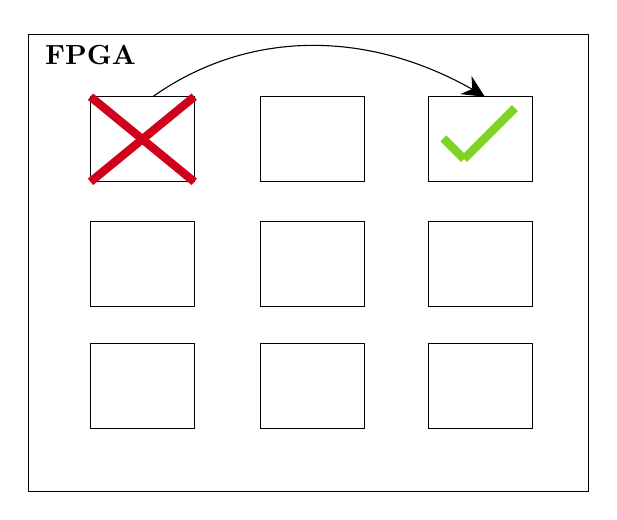
\begin{tikzpicture}[x=0.75pt,y=0.75pt,yscale=-1,xscale=1]
%uncomment if require: \path (0,279); %set diagram left start at 0, and has height of 279

%Shape: Rectangle [id:dp5787797491333819] 
\draw   (6,20) -- (276,20) -- (276,240) -- (6,240) -- cycle ;
%Shape: Rectangle [id:dp17505095690594463] 
\draw   (36,50) -- (86,50) -- (86,91) -- (36,91) -- cycle ;
%Shape: Rectangle [id:dp3058047377979807] 
\draw   (36,110) -- (86,110) -- (86,151) -- (36,151) -- cycle ;
%Shape: Rectangle [id:dp004684645465554249] 
\draw   (36,169) -- (86,169) -- (86,210) -- (36,210) -- cycle ;
%Shape: Rectangle [id:dp3077757040785931] 
\draw   (118,50) -- (168,50) -- (168,91) -- (118,91) -- cycle ;
%Shape: Rectangle [id:dp7450799349257811] 
\draw   (118,110) -- (168,110) -- (168,151) -- (118,151) -- cycle ;
%Shape: Rectangle [id:dp2725857150503048] 
\draw   (118,169) -- (168,169) -- (168,210) -- (118,210) -- cycle ;
%Shape: Rectangle [id:dp3816815123242099] 
\draw   (199,50) -- (249,50) -- (249,91) -- (199,91) -- cycle ;
%Shape: Rectangle [id:dp2885393682660524] 
\draw   (199,110) -- (249,110) -- (249,151) -- (199,151) -- cycle ;
%Shape: Rectangle [id:dp4969175268738504] 
\draw   (199,169) -- (249,169) -- (249,210) -- (199,210) -- cycle ;
%Straight Lines [id:da8580754234796655] 
\draw [color={rgb, 255:red, 208; green, 2; blue, 27 }  ,draw opacity=1 ][line width=3]    (36,50) -- (86,91) ;


%Straight Lines [id:da5772916268060835] 
\draw [color={rgb, 255:red, 208; green, 2; blue, 27 }  ,draw opacity=1 ][line width=3]    (86,50) -- (36,91) ;


%Curve Lines [id:da5702734861080319] 
\draw    (66,50) .. controls (112.04,17.33) and (171.3,17) .. (224.39,49.02) ;
\draw [shift={(226,50)}, rotate = 211.67000000000002] [fill={rgb, 255:red, 0; green, 0; blue, 0 }  ][line width=0.75]  [draw opacity=0] (10.72,-5.15) -- (0,0) -- (10.72,5.15) -- (7.12,0) -- cycle    ;

%Straight Lines [id:da7282259837027933] 
\draw [color={rgb, 255:red, 126; green, 211; blue, 33 }  ,draw opacity=1 ][line width=3]    (240.5,55.5) -- (216,80) ;


%Straight Lines [id:da7142424530641487] 
\draw [color={rgb, 255:red, 126; green, 211; blue, 33 }  ,draw opacity=1 ][line width=3]    (216,80) -- (206,70) ;



% Text Node
\draw (36,30) node  [align=left] {\textbf{FPGA}};


\end{tikzpicture}
}
    \caption{Internal Fault Mitigation - functionality from a faulty tile is moved to a healthy area with \gls{DPR}}\label{fig:internalFaultMitigation}
\end{figure}

%\tikzset{every picture/.style={line width=0.25pt}} %set default line width to 0.75pt        

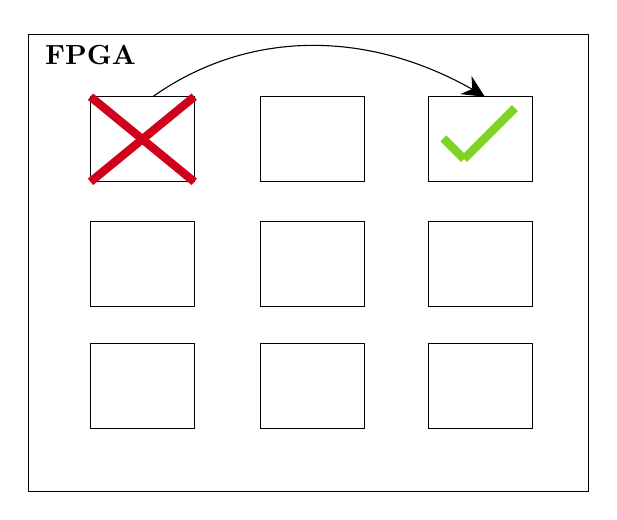
\begin{tikzpicture}[x=0.75pt,y=0.75pt,yscale=-1,xscale=1]
%uncomment if require: \path (0,279); %set diagram left start at 0, and has height of 279

%Shape: Rectangle [id:dp5787797491333819] 
\draw   (6,20) -- (276,20) -- (276,240) -- (6,240) -- cycle ;
%Shape: Rectangle [id:dp17505095690594463] 
\draw   (36,50) -- (86,50) -- (86,91) -- (36,91) -- cycle ;
%Shape: Rectangle [id:dp3058047377979807] 
\draw   (36,110) -- (86,110) -- (86,151) -- (36,151) -- cycle ;
%Shape: Rectangle [id:dp004684645465554249] 
\draw   (36,169) -- (86,169) -- (86,210) -- (36,210) -- cycle ;
%Shape: Rectangle [id:dp3077757040785931] 
\draw   (118,50) -- (168,50) -- (168,91) -- (118,91) -- cycle ;
%Shape: Rectangle [id:dp7450799349257811] 
\draw   (118,110) -- (168,110) -- (168,151) -- (118,151) -- cycle ;
%Shape: Rectangle [id:dp2725857150503048] 
\draw   (118,169) -- (168,169) -- (168,210) -- (118,210) -- cycle ;
%Shape: Rectangle [id:dp3816815123242099] 
\draw   (199,50) -- (249,50) -- (249,91) -- (199,91) -- cycle ;
%Shape: Rectangle [id:dp2885393682660524] 
\draw   (199,110) -- (249,110) -- (249,151) -- (199,151) -- cycle ;
%Shape: Rectangle [id:dp4969175268738504] 
\draw   (199,169) -- (249,169) -- (249,210) -- (199,210) -- cycle ;
%Straight Lines [id:da8580754234796655] 
\draw [color={rgb, 255:red, 208; green, 2; blue, 27 }  ,draw opacity=1 ][line width=3]    (36,50) -- (86,91) ;


%Straight Lines [id:da5772916268060835] 
\draw [color={rgb, 255:red, 208; green, 2; blue, 27 }  ,draw opacity=1 ][line width=3]    (86,50) -- (36,91) ;


%Curve Lines [id:da5702734861080319] 
\draw    (66,50) .. controls (112.04,17.33) and (171.3,17) .. (224.39,49.02) ;
\draw [shift={(226,50)}, rotate = 211.67000000000002] [fill={rgb, 255:red, 0; green, 0; blue, 0 }  ][line width=0.75]  [draw opacity=0] (10.72,-5.15) -- (0,0) -- (10.72,5.15) -- (7.12,0) -- cycle    ;

%Straight Lines [id:da7282259837027933] 
\draw [color={rgb, 255:red, 126; green, 211; blue, 33 }  ,draw opacity=1 ][line width=3]    (240.5,55.5) -- (216,80) ;


%Straight Lines [id:da7142424530641487] 
\draw [color={rgb, 255:red, 126; green, 211; blue, 33 }  ,draw opacity=1 ][line width=3]    (216,80) -- (206,70) ;



% Text Node
\draw (36,30) node  [align=left] {\textbf{FPGA}};


\end{tikzpicture}

\glspl{FPGA} provide high flexibility and good performance in many areas that require a high amount of concurrent computing and therefore benefit from a dedicated hardware implementation.
These properties prove useful for applications in the domain of aerospace and help to reduce the cost for satellites and spacecraft while providing high flexibility throughout the development process. 

But \glspl{FPGA} are especially vulnerable to cosmic radiation which can create a multitude of internal errors in the \gls{FPGA} and thereby breaking its intended functionality \cite{ito_total_2015}.
While there are radiation hardened \glspl{FPGA} available on the market, the mass of a space embedded system is still composed of 80\% radiation shielding \cite{ito_total_2015}.
Yet, this shielding is still not able to provide sufficient protection from radiation induced errors, especially on long term missions. 
Therefore, solutions for fault mitigation in aerospace \glspl{FPGA} need to be developed on the architectural level instead of the physical level. 
This may also provide the advantage of lower requirements for radiation shielding and therefore a reduced cost for payload on rocket launches.

The next section reviews the different types of faults and categorizes them. 

\subsection{Types of Internal Faults}
There are different types of faults that may occur in the lifetime of an \gls{FPGA}, a short overview over the most relevant ones is given in the following.
\par
\textbf{Transient Faults}
\begin{itemize}
    \item \glspl{SEU}, e.g. radiation induced \cite{alkady_fault-tolerant_2014}, \cite{lee_fault-tolerant_2017}
    \begin{itemize}
    \item Change of logic state in memory cell
    \item Commonly tackled by redundancy
    \item Built-in fault detection unit possible
    \end{itemize}
    \item Single Bit Errors (SBEs)
    \item Single Event Transients (SETs)
    \item Address Decoding Faults
\end{itemize}

Faults occur either in the interconnect of the \gls{FPGA} (which uses up to 80\% of the available silicon) or in its actual logic blocks \cite{alkady_fault-tolerant_2014}, \cite{jing_huang_routability_2004}.
\par
\textbf{Permanent Faults}
\begin{itemize}
    \item Time Dependant Dielectric Breakdowns (TDDBs)
    \item Electro Migration
    \item Hot Carrier Effect
\end{itemize}

Based on this review, two main categories of errors emerge.
Firstly, \textit{permanent faults} (also known as \textit{hard errors}), which include all faults that render the affected area completely unusable. 
Secondly, \textit{transient faults} (also known as \textit{soft errors}), which encompasses faults where a reclamation of the erroneous area may still be possible after the initial mitigation process.

\gls{DPR} allows for recovery from both categories.

The following sections introduce the general concept of a fault mitigation- and recovery flow as well as concrete implementations. 

\subsection{Abstract Fault Mitigation Flow}\label{AbstractFaultMitigationFlow}
As the general scheme for fault mitigation is always the same, a brief introduction to the corner stones of every recovery flow is given (depicted in figure \ref{fig:internalFaultFlow}). 

\subsubsection{Detect Fault}
    One key aspect of fault mitigation is fault detection. 
    When faulty behaviour is detected, the origin of the fault needs to be determined.
    Generally, a dedicated (internal or external) control-unit is assigned to the task of result verification.
    This control-unit then gathers information about the location of the affected area and which functionality is corrupted.
\subsubsection{Mitigate Fault}
    After a successful isolation of the fault, steps towards its mitigation are taken.
    Due to external (e.g. increase in radiation) or internal (e.g. space, power)constraints, this stage may encompass some sort of estimation algorithm for the selection of a suitable \gls{PR} block.
    As a consequence, the system can dynamically adapt its fault resistance to changing circumstances.
\subsubsection{Resume Functionality}
    To fully leverage the advantage of \gls{DPR}, some sort of redundancy (e.g. \gls{TMR}) is usually employed.
    This allows the whole system to remain fully functional during the process of \gls{DPR} - the redundant modules will still provide the required data / processing during the reconfiguration. 
    The now freshly instantiated module then needs to re-sync its state with the rest of the system to return to its normal functionality.
\subsubsection{Recover Faulty Area}
    If a transient fault is responsible for the erroneous behaviour, the affected chip area may be recovered by error correction techniques like scrubbing \cite{reorda_error-detection_2017}. 
    In case of a successful recovery, the control-unit can mark the partition as healthy and reuse it at a later point in time.

\begin{center}
\begin{figure}[h]
    \centering
    \resizebox{\smallColumnWidth}{!} {
            \definecolor{one}{HTML}{E52B50}
    %\definecolor{two}{HTML}{fb8072}
    \definecolor{two}{HTML}{80b1d3}
\begin{tikzpicture}[]

\draw[solid]
(-2,0) node[fill=one!20,draw,rounded corners] (B) {Detect Fault}
(1,-1) node[fill=two!20,draw] (C) {Locate Affected Area}
(1,-2) node[fill=two!20,draw] (D) {Determine Affected Functionality}
(1,-3) node[fill=two!20,draw] (E) {Select Suitable PR Block}
(1,-4) node[fill=two!20,draw] (F) {Instantiate PR Block}
(1,-5) node[fill=one!20,draw] (G) {Resume Functionality}
(1,-6) node[fill=two!20,draw] (H) {Recover Faulty Area};
%\draw[dotted] (4, 2) -- (4,-3);
\draw[->, to path={-| (\tikztotarget)}] (B) edge (C);
\draw[->] (C) edge (D);
\draw[->] (D) edge (E);
\draw[->] (E) edge (F);
\draw[->] (F) edge (G);
\draw[->] (G) edge (H);
%\draw[->, to path={-| (\tikztotarget)}] (D) edge (E);
%\draw[->] (E) edge (F);
%\draw[->, to path={-| (\tikztotarget)}] (F) edge (G);
%\draw[->] (G) edge (H);
%\draw[->, to path={-| (\tikztotarget)}] (F) edge (G);
%\draw[->, to path={-| (\tikztotarget)}] (G) edge (H);
%\draw[->, to path={-| (\tikztotarget)}] (H) edge (A);
\draw[->, to path={-| (\tikztotarget)}] (G) edge (B);
\draw[->, to path={-| (\tikztotarget)}] (H) edge (B);
\end{tikzpicture}

    }
\caption{Abstract Fault Mitigation Flow}
\label{fig:internalFaultFlow}
\end{figure}
\end{center}


\subsection{Mitigation Strategies for Internal Faults}\label{MitigationOfInternalFaults}

To mitigate the aforementioned internal faults in an \gls{FPGA}, different strategies can be employed.
All of them feature \gls{DPR} as a means to move functional blocks from a faulty silicon area to a healthy one.
What sets them apart is the way of fault detection and the specifically employed \gls{DPR} strategy.

This section is going to introduce the most common concepts and how they are applied. 

The work in \cite{sharma_run-time_2018} proposes not only ways for fault recovery, but also ways of maintaining as much functionality as possible under varying power constraints. 
\gls{DPR} is utilized to achieve \gls{RT-SA}, i.e. a system that can dynamically alter its architecture to mitigate the effect of changed circumstances.

\section{\gls{DPR} for External Fault Mitigation}\label{ExternalFaults}
Redundancy is a necessary feature to increase the dependability of a system.
Systems that have a need for high dependability encompass e.g. any safety critical system where a fault can result in the harm or even loss of human live.
Systems where maintenance may be difficult or expensive are another set of examples where redundancy is useful.
Redundancy can be achieved through the provision of multiple hardware entities that perform the same task.
If one hardware entity fails, another can take over and supply the expected functionality.
This can get expensive when there are multiple smaller hardware entities that perform specific computational work. 
To reduce space usage and cost, a general purpose \gls{CPU} can be used.
This \gls{CPU} can then emulate the functionality of the faulty hardware and thereby mitigates the fault. 
But this approach introduces new margin for error, as a two-pronged development may lead to discrepancies.
Another issue are real-time requirements that need to be fulfilled.
A regular \gls{CPU} may not be able to provide concurrent computations or the required performance, as the emulated hardware (or software) may be too complex.

A solution to these problems is the usage of \glspl{FPGA} as a means of redundancy. 
As the \gls{FPGA} can be reconfigured with different functionality during runtime, it reduces the total amount of hardware that is needed to achieve redundancy.
Unlike \glspl{CPU}, \glspl{FPGA} provide better means for concurrent computation and are suitable to emulate multiple faulty hardware entities in a more appropriate manner. %TODO: Citation needed

Surprisingly, this approach is not very present in current literature, although the idea is explored by \cite{crdl_fail-safe_nodate} in the year 2002 in the context of \glspl{ECU} for the automotive industry.

The next section will describe the the proposed concept by \cite{crdl_fail-safe_nodate} in more detail.

\subsection{\gls{DPR} for automotive applications}
A fail-safe circuit that is instantiated with \gls{DPR} is presented by \cite{crdl_fail-safe_nodate}. 
This circuit is meant for taking over the real-time functionality of a faulty \gls{ECU} and thereby provides redundancy.
This approach follows the goal of the reduction of hardware costs and the reduction of power and space needs, especially when it is extended to provide multiple backup circuits for different \glspl{ECU}.
One important assumption that is made is that a graceful degradation of performance and functionality is permitted to a certain extent, as long as it does not interfere with the minimal requirements of a safe functionality (e.g. reduction of vehicle speed due to limited processing power).
This is a notable distinction to a fault-tolerant design, which is usually able to mitigate a fault and is still able to fulfil most of its intended functionality.

To achieve redundancy, the \gls{FPGA} is connected to the same bus as the \glspl{ECU} that are monitored.
For each \gls{ECU} a \gls{RP} in the \gls{FPGA} is reserved and hosts a watchdog that monitors the status of the \gls{ECU}.
Through this approach, each \gls{ECU} can be handled individually and a higher resilience against a single point of failure in the monitoring logic is achieved, i.e. the malfunction of one watchdog does not affect the functionality of the others.
When the watchdog registers a fault (i.e. the absence of datagrams from the \gls{ECU}), the backup circuit is instantiated in the same \gls{RP} as the watchdog and overrides its functionality.
The faulty \gls{ECU} tries to shut down all of its communication on the bus and the instantiated backup circuit takes over.
The consumers of the \gls{ECU} should not notice that the data is provided by another entity now. 

This concept was implemented and evaluated for the engine controller (fuel injection) and the transmission controller and was able to achieve the required real-time properties (with a reconfiguration time of 440$\mu$s) for minimal engine-performance.
\begin{figure}
    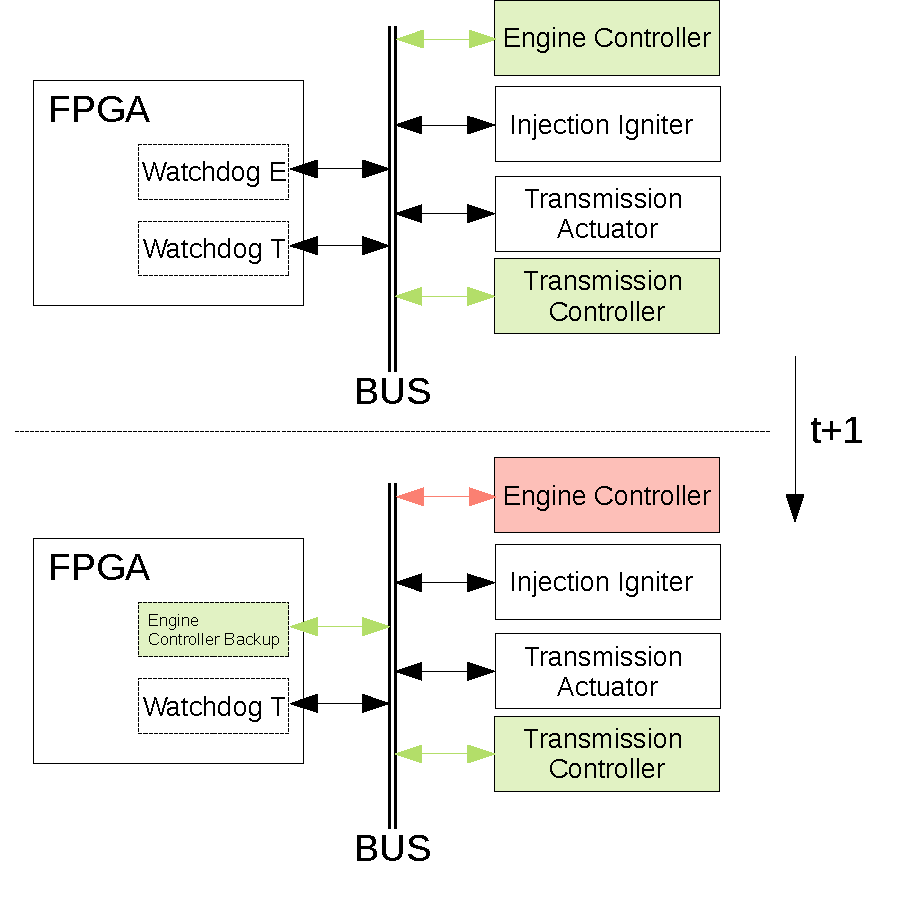
\includegraphics[width=\columnwidth]{./graphics/externalFault.pdf}
    %\resizebox{\columnwidth}{!}{

\tikzset{every picture/.style={line width=0.25pt}} %set default line width to 0.75pt        

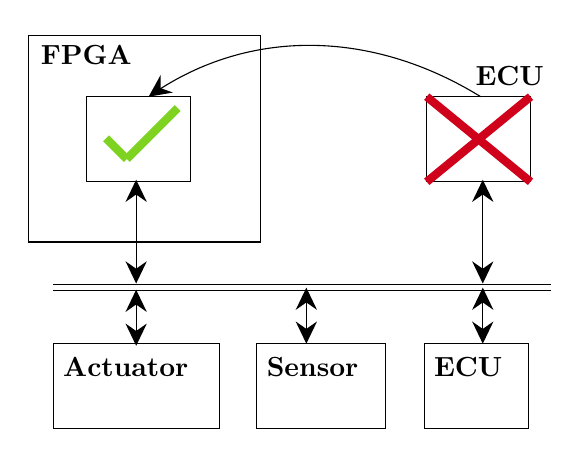
\begin{tikzpicture}[x=0.75pt,y=0.75pt,yscale=-1,xscale=1]
%uncomment if require: \path (0,279); %set diagram left start at 0, and has height of 279

%Shape: Rectangle [id:dp5787797491333819] 
\draw   (8,20.5) -- (120,20.5) -- (120,120) -- (8,120) -- cycle ;
%Shape: Rectangle [id:dp17505095690594463] 
\draw   (36,50) -- (86,50) -- (86,91) -- (36,91) -- cycle ;
%Shape: Rectangle [id:dp004684645465554249] 
\draw   (20,169) -- (100,169) -- (100,210) -- (20,210) -- cycle ;
%Shape: Rectangle [id:dp2725857150503048] 
\draw   (118,169) -- (180,169) -- (180,210) -- (118,210) -- cycle ;
%Shape: Rectangle [id:dp2885393682660524] 
\draw   (200,50) -- (250,50) -- (250,91) -- (200,91) -- cycle ;
%Shape: Rectangle [id:dp4969175268738504] 
\draw   (199,169) -- (249,169) -- (249,210) -- (199,210) -- cycle ;
%Straight Lines [id:da8580754234796655] 
\draw [color={rgb, 255:red, 208; green, 2; blue, 27 }  ,draw opacity=1 ][line width=3]    (200,50) -- (250,91) ;


%Straight Lines [id:da5772916268060835] 
\draw [color={rgb, 255:red, 208; green, 2; blue, 27 }  ,draw opacity=1 ][line width=3]    (250,50) -- (200,91) ;


%Curve Lines [id:da5702734861080319] 
\draw    (68.1,48.54) .. controls (114.3,17.01) and (173.3,17.5) .. (226,50) ;

\draw [shift={(66,50)}, rotate = 324.64] [fill={rgb, 255:red, 0; green, 0; blue, 0 }  ][line width=0.75]  [draw opacity=0] (10.72,-5.15) -- (0,0) -- (10.72,5.15) -- (7.12,0) -- cycle    ;
%Straight Lines [id:da7282259837027933] 
\draw [color={rgb, 255:red, 126; green, 211; blue, 33 }  ,draw opacity=1 ][line width=3]    (80,55.5) -- (55.5,80) ;


%Straight Lines [id:da7142424530641487] 
\draw [color={rgb, 255:red, 126; green, 211; blue, 33 }  ,draw opacity=1 ][line width=3]    (55.5,80) -- (45.5,70) ;


%Straight Lines [id:da36465994520752654] 
\draw    (20,140.5) -- (260,140.5)(20,143.5) -- (260,143.5) ;


%Straight Lines [id:da9447465253235761] 
\draw    (227,92) -- (227,138) ;
\draw [shift={(227,140)}, rotate = 270] [fill={rgb, 255:red, 0; green, 0; blue, 0 }  ][line width=0.75]  [draw opacity=0] (10.72,-5.15) -- (0,0) -- (10.72,5.15) -- (7.12,0) -- cycle    ;
\draw [shift={(227,90)}, rotate = 90] [fill={rgb, 255:red, 0; green, 0; blue, 0 }  ][line width=0.75]  [draw opacity=0] (10.72,-5.15) -- (0,0) -- (10.72,5.15) -- (7.12,0) -- cycle    ;
%Straight Lines [id:da358175601755349] 
\draw    (60,92) -- (60,138) ;
\draw [shift={(60,140)}, rotate = 270] [fill={rgb, 255:red, 0; green, 0; blue, 0 }  ][line width=0.75]  [draw opacity=0] (10.72,-5.15) -- (0,0) -- (10.72,5.15) -- (7.12,0) -- cycle    ;
\draw [shift={(60,90)}, rotate = 90] [fill={rgb, 255:red, 0; green, 0; blue, 0 }  ][line width=0.75]  [draw opacity=0] (10.72,-5.15) -- (0,0) -- (10.72,5.15) -- (7.12,0) -- cycle    ;
%Straight Lines [id:da07393951188629155] 
\draw    (60,145) -- (60,168) ;
\draw [shift={(60,170)}, rotate = 270] [fill={rgb, 255:red, 0; green, 0; blue, 0 }  ][line width=0.75]  [draw opacity=0] (10.72,-5.15) -- (0,0) -- (10.72,5.15) -- (7.12,0) -- cycle    ;
\draw [shift={(60,143)}, rotate = 90] [fill={rgb, 255:red, 0; green, 0; blue, 0 }  ][line width=0.75]  [draw opacity=0] (10.72,-5.15) -- (0,0) -- (10.72,5.15) -- (7.12,0) -- cycle    ;
%Straight Lines [id:da8542656416019287] 
\draw    (142,144) -- (142,167) ;
\draw [shift={(142,169)}, rotate = 270] [fill={rgb, 255:red, 0; green, 0; blue, 0 }  ][line width=0.75]  [draw opacity=0] (10.72,-5.15) -- (0,0) -- (10.72,5.15) -- (7.12,0) -- cycle    ;
\draw [shift={(142,142)}, rotate = 90] [fill={rgb, 255:red, 0; green, 0; blue, 0 }  ][line width=0.75]  [draw opacity=0] (10.72,-5.15) -- (0,0) -- (10.72,5.15) -- (7.12,0) -- cycle    ;
%Straight Lines [id:da22998818326497883] 
\draw    (227,144) -- (227,167) ;
\draw [shift={(227,169)}, rotate = 270] [fill={rgb, 255:red, 0; green, 0; blue, 0 }  ][line width=0.75]  [draw opacity=0] (10.72,-5.15) -- (0,0) -- (10.72,5.15) -- (7.12,0) -- cycle    ;
\draw [shift={(227,142)}, rotate = 90] [fill={rgb, 255:red, 0; green, 0; blue, 0 }  ][line width=0.75]  [draw opacity=0] (10.72,-5.15) -- (0,0) -- (10.72,5.15) -- (7.12,0) -- cycle    ;

% Text Node
\draw (36,30) node  [align=left] {\textbf{FPGA}};
% Text Node
\draw (240,40) node  [align=left] {\textbf{ECU}};
% Text Node
\draw (220,180) node  [align=left] {\textbf{ECU}};
% Text Node
\draw (145,180) node  [align=left] {\textbf{Sensor}};
% Text Node
\draw (55,180) node  [align=left] {\textbf{Actuator}};


\end{tikzpicture}
}
    \caption{External Fault Mitigation - functionality from a faulty \gls{ECU} is provided by a module (instantiated with \gls{DPR}) within the \gls{FPGA}}\label{fig:externalFaultMitigation}
\end{figure}

This guy points out problems \cite{shanker_enhancing_nodate}.
\section{Conclusion}\label{Conclusion}
This paper surveys and identifies the most common concepts that utilize \gls{DPR} in \glspl{FPGA} for fault mitigation.
Common reasons for faults in \glspl{FPGA} are identified and classified into transient faults that allow a full recovery and permanent faults which render the affected area useless. 
We show that these faults allow for mitigation on the architectural level.
The topic is widely researched and many concepts extend architectures that already exist by a fault mitigation feature.
\gls{TMR} is enhanced by the possibility to move faulty modules to healthy spare tiles which greatly increases the lifetime and reliability of the \gls{TMR} architecture.  
Hardware-based task-schedulers already use \gls{DPR} and faults in the \gls{RP} can therefore be handled by an extension of the placement algorithm.
This algorithm can then avoid the faulty area in future placement calculations.
\gls{DPR} enables graceful performance degradation of healthy modules to free up area for a module that resides in a faulty area when no other spare space is available anymore. 
\glspl{NoC} profit from an improved security, as malicious nodes can be disconnected from the network on the routing level through \gls{DPR}.
Corner nodes in \glspl{NoC} that are isolated due to a router failure can be reintegrated into the network by the reconfiguration of link mappings on a healthy router. 
Research with regards to external fault mitigation is still scarce but will gain more traction with the continuous improvement of \glspl{FPGA}, development tools and the creation of standards.
Overall, the usage of \gls{DPR} for fault mitigation is already recognized as a potential solution for many reliability problems but lacks a broader adaption in commercial projects outside the aerospace sector.
Commercial adaption will increase when standardized hardware schedulers and \glspl{NoC} gain popularity as they can easily provide fault mitigation features by design without any extra development effort by the users.

\bibliographystyle{IEEEtran}
\bibliography{IEEEabrv,SocSeminar2}

\end{document}
